\documentclass[output=paper]{LSP/langsci} 
\author{Martin Volk\affiliation{University of Zurich, Institute of Computational Linguistics}\and
Torsten Marek\lastand 
Yvonne Samuelsson\affiliation{Stockholm University, Department of Linguistics}
}
\title{Building and querying parallel treebanks} 
\abstract{This paper describes our work on building a trilingual parallel treebank. We have annotated constituent structure trees from three text genres (a philosophy novel, economy reports and a technical user manual). Our parallel treebank includes word and phrase alignments. The alignment information was manually checked using a graphical tool that allows the annotator to view a pair of trees from parallel sentences. This tool comes with a powerful search facility which supersedes the expressivity of previous popular treebank query engines.}
\maketitle

\begin{document}

%8050 Zurich, Switzerland
%volk@cl.uzh.ch
%106 91 Stockholm, Sweden
%yvonne.samuelsson@ling.su.se

\section{Introduction}\label{sec:volk:1}

Recent years have seen a number of initiatives in building parallel treebanks (see \citealt{Abeillé2003, NivreEtAl2005}). The current interest in treebanks is documented in international workshop series like ``Linguistically Interpreted Corpora (LINC)'' or ``Treebanks and Linguistic Theories'' (TLT). 

We see a treebank as a particular kind of annotated corpus where each sentence is mapped to a special type of graph, a tree which represents its syntactic structure. Traditionally the graphs were constituent structure trees but recent years have also seen dependency treebanks. Constituent structure trees contain nodes and edges where each node holds a label for a group of words (as e.g.~NP for noun phrase or VP for verb phrase). Dependency trees represent syntactic dependencies between words directly. We work with constituent structure trees that have labeled edges to denote functional relations which can easily be mapped to dependencies. The concept of constituent structure trees in treebanking has been stretched beyond proper trees as defined in graph theory by accepting crossing edges and even secondary edges. 

Parallel treebanks are treebanks over parallel corpora, i.e.~the ``same'' text in two or more languages, where one text might be the source text and the other texts are translations thereof, or where all texts are translations of a text outside of the corpus. In addition to the syntactic annotation, a parallel treebank is aligned on the sub-sentential level, for example on the word level or the phrase level. 

Parallel treebanks can be created automatically or manually. Automatic creation entails automatic parsing and automatic alignment, both of which will result in a certain amount of error at the current state of the technology. In this paper we focus on the manual creation of parallel treebanks. 

Parallel treebanks can be used as training or evaluation corpora for word and phrase alignment, as input for example-based machine translation (EBMT), as training corpora for transfer rules, or for translation studies. 

Parallel treebanks have evolved into a research field in the last decade. \citet{CmejrekEtAl2003} at the Charles University in Prague have built a parallel treebank for the specific purpose of machine translation, the Czech-English Penn Treebank with tectogrammatical dependency trees. They have asked translators to translate part of the Penn Treebank into Czech with the clear directive to translate every English sentence with one in Czech and to stay as close as possible to the original. 

Other parallel treebank projects include Croco \citep{Hansen-SchirraEtAl2006} which is aimed at building an English-German treebank for translation studies, LinES an English-Swedish parallel treebank \citep{Ahrenberg2007}, and the English-French HomeCentre treebank \citep{Hearne2006}, a hand-crafted parallel treebank consisting of 810 sentence pairs from a Xerox printer manual. 

Our group has contributed to these efforts by building a tri-lingual parallel treebank called S\textsc{multron} (Stockholm MULtilingal TReebank). Our parallel treebank consists of syntactically annotated sentences in three languages, taken from translated documents. The syntax trees of corresponding sentence pairs are aligned on a sub-sentential level. On the side we have also experimented with building parallel treebanks for the widely differing languages Quechua and Spanish \citep{RiosEtAl2009}. 

In this paper we will first describe our parallel treebank and the difficulties in consistent annotation. We have developed a special alignment tool and present its functionality for alignment and search of parallel treebanks. To our knowledge this is the first dedicated tool that combines visualization, alignment and searching of parallel treebanks. 

\section{Building SMULTRON - The Stockholm MULtilingual TReebank}\label{sec:volk:2}

We have built a trilingual parallel treebank in English, German and Swedish. In its 2008 release S\textsc{multron} consists of around 500 trees from the novel \textit{Sophie's World} and 500 trees from economy texts (an annual report from a bank, a quarterly report from an international engineering company, and the banana certification program of the Rainforest Alliance) \citep{Samuelsson2006, Samuelsson2007}. The sentences in Sophie's World are relatively short (14.8 tokens on average in the English version), while the sentences in the economy texts are much longer (24.3 tokens on average; 5 sentences in the English version have more than 100 tokens). 

Lately we have added 500 trees from another text genre: a user manual for a DVD player. This genre differs in that it contains a multitude of imperative constructions, many numerical expressions as well as many itemized and enumerated lists. S\textsc{multron} version 2.0 consisting of 1500 trees from three text genres in three languages has been released in the beginning of 2010.\footnote{S\textsc{multron} is freely available from http://kitt.cl.uzh.ch/kitt/smultron/}

\subsection{Monolingual treebanking}\label{sec:volk:2.1}

For English and German, there are large monolingual treebanks that have resulted in standards for treebanking in these languages. We have followed these standards and (semi-automatically) annotated the German sentences of our treebank with Part-of-Speech tags and phrase structure trees (incl.~edges labeled with functional information) according to the NEGRA guidelines \citep{BrantsEtAl1997}. 

For English, we have used the Penn Treebank guidelines which also prescribe phrase structure trees (with PoS tags, but only partially annotated with functional labels). However they differ from the German guidelines in many details. For example, the German trees use crossing edges for discontinuous units while the English trees introduce symbols for empty tokens plus secondary edges for the representation of such phenomena. 

There has been an early history of treebanking in Sweden, dating back to the 1970s (cf.~\citealt{Nivre2002}. The old annotation schemes were difficult for automatic processing (in the case of Talbanken, \citealt{Teleman1974})\footnote{Talbanken has recently been cleaned and converted to a dependency treebank by Joakim Nivre and his group. See http://w3.msi.vxu.se/~nivre/research/talbanken.html} or too coarse-grained (in the case of Syntag, \citealt{Järborg1986}). Therefore we have developed our own treebanking guidelines for Swedish inspired by the German guidelines. 

We annotated the treebanks for all three languages separately, with the help of the treebank editor A\textsc{nnotate}\footnote{Annotate is a treebank editor developed at the University of Saarbrücken. See http://www.coli.uni-sb.de/sfb378/negra-corpus/annotate.html}. A\textsc{nnotate} includes the TnT Part-of-Speech Tagger and Chunker for German. We added taggers and chunkers for Swedish and English. After finishing the monolingual treebanks, the trees were exported from the accompanying SQL database and converted into an XML format as input to our alignment tool, the TreeAligner. 

Both the German trees and the Swedish trees are annotated with flat structures but subsequently automatically deepened to result in richer and linguistically more plausible tree structures. 

\subsubsection{Automatic treebank deepening}\label{sec:volk:2.1.1}

The German NEGRA annotation guidelines \citep{BrantsEtAl1997} result in rather flat phrase structure trees. This means, for instance, no unary nodes, no ``unnecessary'' NPs (noun phrases) within prepositional phrases and no finite verb phrases. Using a flat tree structure for manual treebank annotation has two big advantages for the human annotator: 1) the annotator needs to make fewer decisions, and 2) the annotator has a better overview of the trees. This comes at the cost of the trees not being complete from a linguistic point of view. One could ask why an NP that consists of only one daughter is not marked, or why an NP that is part of a PP is not marked, while the same NP outside a PP is explicitly annotated. These restrictions also have practical consequences: If certain phrases (e.g.~NPs within PPs) are not explicitly marked, then they can only indirectly be searched in corpus linguistics studies. 

In addition to the linguistic drawbacks of the flat syntax trees, they are also problematic for phrase alignment in a parallel treebank. Our goal is to align sub-sentential units (such as phrases and clauses) to get fine-grained correspondences between languages. The alignment focuses on meaning, rather than sentence structure. For example, sentences can have alignment on a higher level of the tree (for instance, if the sentence carries the same meaning in both languages), without necessarily having alignment on all lower levels (for instance, if the sentence contains an NP without direct correspondence in the other language). We prefer to have ``deep trees'' to be able to draw the alignment between the German sentences and the parallel Swedish sentences on as many levels as possible; in fact, the more detailed the sentence structure is, the more expressive is our alignment. 

We deepened the flat phrase structure trees automatically with a script, which automatically inserts nodes to create the deeper structure. However, these insertions must be totally unambiguous, so that no errors are introduced. The input for this program is a tree description in TIGER-XML \citep{König2002}, an interface format which can be created and used by the treebank tool TIGERSearch\footnote{See also http://www.ims.uni-stuttgart.de/projekte/TIGER.}. The output is a deepened TIGER-XML tree. We have measured that the automatic node insertion resulted in an increase of almost 60\% additional nodes. 

\subsubsection{Completeness and consistency checks over treebanks}\label{sec:volk:2.1.2}

Completeness and consistency are important characteristics of corpus annotation. Tree completeness means that each token and each node is part of the tree.\footnote{Different treebanks take different positions on whether special tokens like punctuation symbols should be part of the tree. For example, the Penn Treebank guidelines require punctuation marks to be part of the tree, whereas the German TIGER guidelines leave them unattached.} This can easily be checked and should ideally be part of the annotation tool. 

Consistency checking is more complicated. Consistent annotation means that the same token sequence (or part-of-speech sequence or phrase sequence) is annotated in the same way across the treebank. Annotation error detection has been explored for part-of-speech annotation \citep{Dickinson2003a,Loftsson2009} and syntactic annotation \citep{Ule2004,Dickinson2005}. 

The variation \textit{n}{}-gram approach for syntactic annotation \citep{Dickinson2003b, Dickinson2005} is a method for detecting strings which occur multiple times in the corpus with varying annotation. The approach can detect bracketing and labeling errors in constituency annotation. 

\subsection{Aligning trees}\label{sec:volk:2.2}

Establishing translation correspondences is a difficult task. This task is traditionally called alignment and is usually performed on the paragraph level, sentence level and word level. Alignment answers the question: Which part of a text in language L1 corresponds in meaning to which part of a text in language L2 (under the assumption that the two texts represent the same meaning in different languages)? 

There is considerable interest in automating the alignment process. Automatic sentence alignment of legacy translations helps to fill translation memories. Automatic word alignment is a crucial step in training statistical machine translation systems. Both sentence and word alignment have to deal with 1-to-many alignments, e.g.~sometimes a sentence in one language is translated as two or three sentences in the other language. 

In other respects sentence alignment and word alignment are fundamentally different. It is relatively safe to assume the same sentence order in both languages when computing sentence alignment. But such a monotonicity assumption is not possible for word alignment which needs to allow for word order differences and thus for crossing alignments. While basic algorithms for sentence alignment can rely on unsophisticated measures like sentence length in characters and still produce good results, word alignment algorithms use cross-language cooccurrence frequencies as a key feature. 

Our work focuses on word alignment and on an intermediate alignment level which we call \textbf{phrase} \textbf{alignment}. Phrase alignment encompasses the alignment from simple noun phrases and prepositional phrases all the way to complex clauses. For example, on the word alignment level we want to establish the correspondence of the German ``verb form plus separated prefix'' \textit{fing an} with the English verb form \textit{began}. In phrase alignment, we mark the correspondence of the verb phrases \textit{ihn in den Briefkasten gesteckt }and \textit{dropped it in the mail box}. For the alignment we have developed a specific tool called TreeAligner \citep{LundborgEtAl2007}, which displays two trees and allows the user to draw alignment lines by clicking on phrases and words. 

We regard phrase alignment as alignment between linguistically motivated phrases, in contrast to work in statistical machine translation where phrase alignment is defined as the alignment between arbitrary consecutive word sequences. Our phrase alignment is alignment between nodes in constituent structure trees. See \figref{fig:volkmareksamuelsson:1} for an example of a tree pair with word and phrase alignment. Green lines indicate exact alignments and red lines represent fuzzy alignments (cf.\sectref{sec:volk:2.2.2}). 

\largerpage
We believe that linguistically motivated phrase alignment provides useful phrase pairs for example-based machine translation, and provides interesting insights for translation science and cross-language comparisons. Phrase alignments are particularly useful for annotating correspondences of idiomatic or metaphoric language use. 

\subsubsection{Related research}\label{sec:volk:2.2.1}

Our research on word and phrase alignment is related to previous work on word alignment as e.g.~in the Blinker project \citep{Melamed1998} or in the UPLUG project \citep{AhrenbergEtAl2003}. Alignment work on parallel treebanks is rare. Most notably there is the Prague Czech-English treebank \citep{Kruijff-KorbayováEtAl2006} and the Linköping Swedish-English treebank \citep{Ahrenberg2007}. There has not been much work on the alignment of linguistically motivated phrases. \citet{TinsleyEtAl2007} and \citet{GrovesEtAl2004} report on semi-automatic phrase alignment as part of their research on example-based machine translation. 

The most comprehensive study is probably the recent PhD thesis by \citet{Zhechev2009}. The author describes his system for automatic phrase alignment over parallel trees which is based on word alignment probabilities provided by GIZA. He evaluates his system against the manually aligned HomeCentre treebank and reports on about 78\% recall for 80\% precision. These results are comparable to \citet{Ambati2008}. These approaches are unsupervised in the sense that human-aligned trees are used only for evaluation. 

\begin{figure}
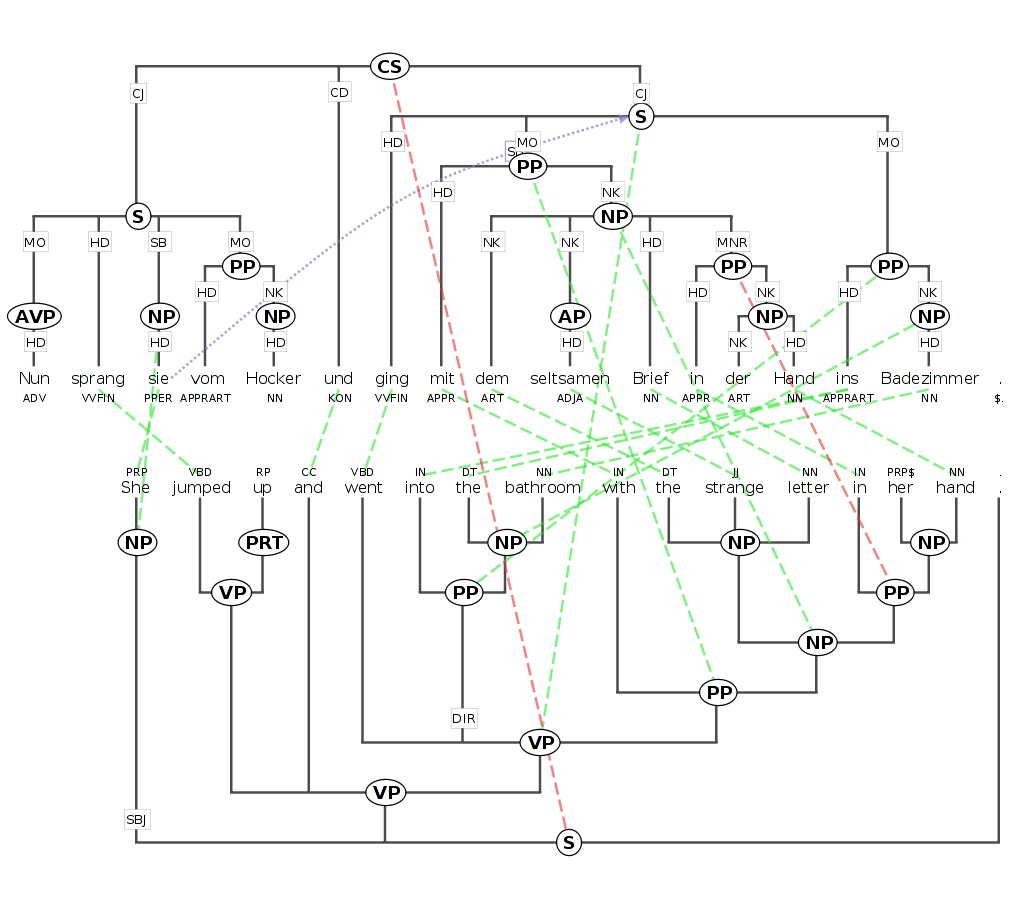
\includegraphics[width=\textwidth]{figures/VolkMarekSamuelssonF1.png}
\caption{Three pair German-English with word and phrase alignments.}
\label{fig:volkmareksamuelsson:1}
\end{figure}

\citet{Tiedemann2009} present a supervised approach which automatically learns phrase alignment features from our parallel treebank. By training on 400 aligned trees and testing on the remaining 100, they report on 80\% precision and 76\% recall. 


Considering the fact that the alignment task is essentially a semantic annotation task, we may also compare our work to other tasks in semantic corpus annotation, for example, the frame-semantic annotation in the German SALSA project (cf.~\citealt{BurchardtEtAl2006}).

\subsubsection{Our alignment guidelines}\label{sec:volk:2.2.2}

We have compiled alignment guidelines for word and phrase alignment between annotated syntax trees. The guidelines consist of general principles, concrete rules and guiding principles. The most important general principles are: 

\begin{enumerate}
\item Align items that can be re-used as units in a machine translation system. 
\item Align as many items (i.e.~words and phrases) as possible. 
\item Align as close as possible to the tokens.
\end{enumerate} 

The first principle is central to our work. The focal point is whether a phrase pair is general enough to be re-used as translation unit in a machine translation system. For example, in our Sophie's World treebank we have decided not to align \textit{die Verwunderung über das Leben} with \textit{their astonishment at the world} although these two phrases were certainly triggered by the same phrase in the Norwegian original, and both have a similar function in the two corresponding sentences. These two phrases in isolation are too far apart in meaning to license their re-use. We are looking for correspondences like \textit{was für eine seltsame} \textit{Welt }and \textit{what an extraordinary world }which would make for a good translation in many other contexts. 

Some special rules follow from this principle. For example, we have decided that a pronoun in one language shall never be aligned with a full noun in the other, since such a pair is not directly useful in a machine translation system. 

\newpage 
Principles 2 and 3 are more technical. Principle 2 tells our annotators that alignment should be comprehensive. We want to re-use as much as possible from the treebank, so we have to look for as many alignments as possible. Principle 3 says that in case of doubt the alignment should go to the node that is closest to the terminals. For example, our German treebank guidelines require a multi-word proper noun to first be grouped in a PN phrase which is a single daughter node of a noun phrase [[Sofie Amundsen]PN ]NP. When we align the name, principle 3 tells us to draw the alignment line from the German PN node since it is closer to the tokens than the German NP node. 

Often we are confronted with phrases that are not exact translation correspondences but approximate translation correspondences. Consider the phrases \textit{mehr als eine Maschine} and \textit{more than a piece of hardware}. This pair does not represent the closest possible translation, but it represents a possible translation in many contexts. In a way we could classify this pair as the ``second-best'' translation. To allow for such distinctions we provide our annotators with a choice between exact translation correspondences and approximate correspondences. We also use the term \textbf{fuzzy correspondence} to refer to and give an intuitive picture of these approximate correspondences. The option to distinguish between different alignment strengths sounded very attractive at the start. But where and how can we draw the line between exact and fuzzy translation correspondences? We have formulated some clear-cut rules: 

\begin{itemize}
\item 
If an acronym is to be aligned with a spelled-out term, it is always an approximate alignment. For example, in our economy reports the English acronym \textit{PT} stands for \textit{Power Technology} and is aligned to the German \textit{Energietechnik} as a fuzzy correspondence. 
\item  
Proper names shall be aligned as exact alignments (even if they are spelled differently across languages; e.g.~\textit{Sofie} vs. \textit{Sophie}).
\end{itemize} 

But many open questions persist. Is \textit{einer der ersten Tage im Mai }an exact or rather a fuzzy translation correspondence of \textit{early May}? We decided that it is not an exact correspondence. How shall we handle \textit{zu dieser} \textit{Jahreszeit} vs.~\textit{at this time of the year }where a literal translation would be \textit{in this season}? We decided that the former is still an exact correspondence. These examples illustrate the difficulties in distinguishing between exact and approximate translation correspondence. 
\
Automatically ensuring the overall consistency of the alignment decisions is a difficult task. We have built a tool to ensure the consistency within the exact and approximate alignment classes. The tool computes the token span for each alignment and checks if the same token span pairs have always received the same alignment type. For example, if the phrase pair \textit{mit einer blitzschnellen Bewegung} and \textit{with a} \textit{lightning movement} is once annotated as exact alignment, then it should always be annotated as exact alignment. \figref{fig:volkmareksamuelsson:1} shows approximate alignments between the PPs \textit{in der Hand }and \textit{in her hand}. It was classified as approximate rather than exact alignment since the German PP lacks the possessive determiner. 

Currently our alignment guidelines are more than 15 pages long with examples for English-German and English-Swedish alignments. The challenge was to compile precise and comprehensive guidelines to ensure smooth and consistent alignment decisions. In \citet{Samuelsson2006} we have reported on experiments to evaluate inter-annotator agreement from our alignment tasks. Here we summarize an experiment described in detail in \citet{Volk2008} in which we evaluated our alignment guidelines. 

\subsubsection{Inter-annotator agreement experiments}\label{sec:volk:2.2.3}

In order to evaluate the inter-annotator agreement for the alignment task we performed the following experiment. We gave 20 tree pairs in German and English to 12 advanced undergraduate students. Half of the tree pairs were taken from our Sophie's World treebank and the other half from our Economy treebank. We made sure that there was one 1-to-2 sentence alignment in the sample. The students did not have access to the gold standard alignment. 

In class we demonstrated the alignment tool to the students, and we introduced the general alignment principles to them. Then the students were given a copy of the alignment guidelines. We asked them to do the alignments independently of each other and to the best of their knowledge according to the guidelines. 

\begin{table}
\begin{tabular}{llrrr} 
\lsptoprule
& \bfseries Alignment Type & \bfseries exact & \bfseries fuzzy & \bfseries total\\
\midrule
Sophie part & word alignment & 75 & 3 & 78 \\
& phrase alignment & 46 & 12 & 58 \\
Economy part & word alignment & 159 & 19 & 178 \\
& phrase alignment & 62 & 9 & 71 \\
\lspbottomrule
\end{tabular}
\caption{Alignment Frequencies in the Gold Standard}
\label{tab:volkmareksamuelsson:1}
\end{table}


Our own annotation of the 20 tree pairs (the gold standard alignment) contains the alignments shown in \tabref{tab:volkmareksamuelsson:1}. In the Sophie part of the experiment treebank we have 78 word-to-word alignments and 58 phrase-to-phrase alignments. Note that some phrases consist only of one word and thus the same alignment information is represented twice. We have deliberately kept this redundancy. 

The alignments in the Sophie part consist of 125 times 1-to-1 alignments, 4 times 1-to-2 alignments and one 1-to-3 alignment (\textit{wäre }vs.~\textit{would have been}) when viewed from the German side. There are 3 times 1-to-2 alignments (e.g.~\textit{introducing }vs.~\textit{stellte vor}) and no other 1:many alignment when viewed from the English side. In the Economy part the picture is similar. 

The student alignments showed a huge variety in terms of numbers of alignments. In the Sophie part they ranged from 125 alignments to bare 47 alignments (exact alignments and fuzzy alignments taken together). In the Economy part, the variation was between 259 and 62 alignments. On closer inspection we found that the student with the lowest numbers works as a translator and chose to use a very strict criterion of translation equivalence rather than translation correspondence. Three other students at the end of the list were not native speakers of either German or English. We therefore decided to exclude these 4 students from the following comparison. 

The student alignments allow for the investigation of a number of interesting questions: 

\begin{itemize}
\item How did the students' alignments differ from the gold standard? 
\item Which were the alignments done by all students? 
\item Which were the alignments done by single students only? 
\item Which alignments varied most between exact and fuzzy alignment?
\end{itemize}

\subsubsection{Inter-annotator agreement results}\label{sec:volk:2.2.4}

The remaining 8 students reached between 81\% and 48\% overlap with our gold standard on the Sophie part, and between 89\% and 66\% overlap with our gold standard on the Economy texts. This can be regarded as their recall values if we assume that the gold standard represents the correct alignments. These students additionally had between 2 and 22 own alignments in the Sophie part and between 12 and 55 own alignments in the Economy part. 

So the interesting question is: What kind of alignments have they missed, and which were the additional own alignments that they suggested (alignments that are not in the gold standard)? We first checked the students with the highest numbers of own alignments. We found that some of these alignments were due to the fact that students had ignored the rule to align as close to the tokens as possible (principle 3 above). 

Another reason was that students sometimes aligned a word (or some words) with a node. For example, one student had aligned the word \textit{natürlich }to the phrase \textit{of course }instead of to the word sequence \textit{of course}. Our alignment tool allows that, but the alignment guidelines discourage such alignments. There might be exceptional cases where a word-to-phrase alignment is necessary in order to keep valuable information, but in general we try to stick to word-to-word and phrase-to-phrase alignments. 

Another discrepancy occurred when the students aligned a German verb group with a single verb form in English (e.g.~\textit{ist zurückzuführen }vs.~\textit{reflecting}). We have decided to only align the full verb to the full verb (independent of the inflection). This means that we align only \textit{zurückzuführen} to \textit{reflecting }in this example. 

The uncertainties on how to deal with different grammatical forms led to the most discrepancies. Shall we align the definite NP \textit{die Umsätze }with the indefinite NP \textit{revenues }since it is much more common to drop the article in an English plural NP than in German? Shall we align a German genitive NP with an of-PP in English (\textit{der beiden }\textit{Divisionen }vs.~\textit{of the two divisions})? We have decided to give priority to form over function and thus to align the NP \textit{der beiden Divisionen }with the NP \textit{the two divisions}. But of course this choice is debatable. 

When we compute the \textbf{intersection }of the alignments done by all students (ignoring the difference between exact and fuzzy alignments), we find that about 50\% of the alignments done by the student with the smallest number of alignments is shared by all other students. All of the alignments in the intersection are in our gold standard file. This indicates that there is a core of alignments that are obvious and uncontroversial. Most of them are word alignments. 

When we compute the \textbf{union }of the alignments done by all students (again ignoring the difference between exact and fuzzy alignments), we find that the number of alignments in the union is 40\% to 50\% higher than the number of alignments done by the student with the highest number of alignments. It is also about 40\% to 50\% higher than the number of alignments in the gold standard. This means that there is considerable deviation from the gold standard. 

Other discrepancies concern cases of differing grammatical forms, e.g.~a German definite singular noun phrase (\textit{die Hand}) that was aligned to an English plural noun phrase (\textit{hands}) in the gold standard but missed by all students. Finally there are a few cases where obvious noun phrase correspondences were simply overlooked by all students (\textit{sich - herself}) although the tokens themselves were aligned. Such cases should be handled by an automated process in the alignment tool that projects from aligned tokens to their mother nodes (in particular in cases of single token phrases). 

\subsubsection{Working with the TreeAligner}\label{sec:volk:2.2.5}

The tree alignments in S\textsc{multron} and in the experiments above were done with a tool called TreeAligner. Let us look at the alignment process in more detail. 

When our monolingual treebanks were finished, the trees were exported from the editor system and converted into TIGER-XML, an XML format for encoding syntax graphs with crossing dominance branches and secondary edges. TIGER-XML has been defined as input format for TIGERSearch, a query tool for monolingual treebanks (see \sectref{sec:volk:3.1}). We use TIGER-XML also as input format for the TreeAligner \citep{VolkEtAl2006}. 

The TreeAligner program is a graphical user interface to specify (or correct) word and phrase alignments between pairs of syntax trees. \footnote{The TreeAligner was implemented in Python by Joakim Lundborg and Torsten Marek. It is freely available at http://www.cl.uzh.ch/treealigner.html} The TreeAligner is roughly similar to alignment tools such as I*Link \citep{AhrenbergEtAl2002} or Cairo \citeauthor{Smith2000} it is especially tailored to visualize and align full syntax trees. The TreeAligner is unique in that it allows the alignments of linguistically motivated phrases via node alignments in parallel constituent structure trees (cf.~\citealt{Samuelsson2007}). 

The TreeAligner operates on an alignment file in an XML format developed by us. This file describes the alignments between two TIGER-XML treebanks (specified in the alignment file) holding the trees from language one and language two respectively. For example the alignment between two nodes is represented as: 

\ea
\begin{lstlisting}
<align type="good"> 
  <node treebank_id="de" node_id="s153_11"/> 
  <node treebank_id="en" node_id="s144_10"/> 
</align>
\end{lstlisting}
\z 

This says that node 11 in sentence 153 of the German treebank (de) is aligned with node 10 in sentence 144 of the English treebank (en). The node identifiers refer to the IDs in the TIGER-XML treebanks. The alignment is given the label ``good'' or ``fuzzy'' depending on the degree of meaning correspondence. 


The alignment file might initially be empty when we start manual alignment from scratch, or it might contain automatically computed alignments for correction. The TreeAligner displays tree pairs with the trees in mirror orientation (one top-up and one top-down) exemplified in \figref{fig:volkmareksamuelsson:1}. The trees are displayed with node labels, edge labels and part-of-speech tags. 

Each alignment is displayed as a dotted line between two nodes (or words) across two trees. Clicking on a node (or a word) in one tree and dragging the mouse pointer to a node (or a word) in the other tree inserts an alignment line. The type of the alignments is represented by its color. Our experiments indicate that eventually more alignment types than just the two used in S\textsc{multron} will be needed to precisely represent fine-grained translation differences. In its most recent version, the TreeAligner supports arbitrarily many alignment types, which can describe many different levels or modes of alignment. These distinctions could prove useful when exploiting the aligned treebanks for Machine Translation and other applications. 

Often one tree needs to be aligned to two (or more) trees in the other language. The TreeAligner therefore provides the option to browse the trees independently. 

The TreeAligner is designed as a stand-alone tool (i.e.~it is not prepared for collaborative annotation). It stores every alignment in an XML file (in the format described above) as soon as the user moves to a new tree pair. 

Lately, we have included an interactive module that suggests word and phrase alignments. It follows an alignment memory strategy in analogy to translation memories. This means that the module stores each alignment made by the human annotator. If a new tree pair is to be aligned, the module checks whether any token sequence in the current trees has been previously aligned. If so, it suggests the stored alignment to the annotator. 

\subsubsection{Consistency checks over alignments}\label{sec:volk:2.2.6}

Based on the lessons learned in the inter-annotator agreement experiments, we have improved our alignment guidelines. The question is how we can ensure that the guidelines are followed. We would like to determine whether the alignments are complete and consistent, in similarity to quality checks over treebanks. 

For consistency checking of the alignments, we checked for all aligned single tokens and all aligned token sequences whether they are aligned in the same way (i.e. with the predicate `exact' or `fuzzy') to the same corresponding tokens. We also checked whether the aligned token sequences differ in length (calculated as number of characters). Large length differences point to possibly erroneous alignments. 

Additionally, we examined those cases where different types of nodes are aligned across the languages (e.g., when an adjective phrase in one language is aligned with a prepositional phrase in the other). These consistency checks were initially done manually over an extracted table of the aligned token sequences (with their node labels). This allowed us to sort the token sequences according to different criteria and to abstract away from the dense forest of syntactic information and alignment lines in the TreeAligner. 

In order to provide faster feedback about internal alignment link consistency, recent versions of the TreeAligner contain a module for consistency checks that are computed during annotation. We distinguish between two different methods, general structural constraints and association probability. Structural constraints are applied regardless of language or corpus, as they express certain invalid subgraphs. One structural constraint that has proven useful to the annotators is branch link locality, which demands that if two phrases \textit{p}\textsubscript{1}\textit{, p}\textsubscript{2} are aligned, any transitive successor of \textit{p}\textsubscript{1} may only be aligned to a successor of \textit{p}\textsubscript{2}. While there are some systematic problems with this constraint, it is very effective in exposing inconsistencies among the monolingual annotations and spotting simple mistakes. 
 
The other approach relies on measuring association strength between collocates. In our case, we define an alignment link to be our collocate and check if, given the totality of all alignment links in the current corpus, we can reject it as an improbable hypothesis. For this, we use contingency tables and a \textit{$\chi $}\textsuperscript{2} statistic for non-parametric data. 
 
Another (forthcoming) method for consistency checking of alignment draws on the variation \textit{n}{}-gram approach for syntactic annotation \citep{Dickinson2003b,Dickinson2005}. It considers alignment as a string-to-string mapping and, treating the target string as a label, examines each source string and their labels, to find inconsistencies in the alignment. Several heuristics are used to filter the set of variations, based on source language context and based on the nature of alignments in aligned corpora. One additional, complementary, method predicts what phrasal node (if any) a constituent should be aligned to, based on the word alignment. 

\section{Searching parallel treebanks}\label{sec:volk:3}

Since the inception of treebanks, many languages and tools for querying syntactically annotated corpora have been developed. Most of the tools and query languages have been designed for a specific corpus and a specific annotation format. 

Our survey focuses on TGrep and TIGERSearch since they were most influential for our own work. We are well aware of related approaches on searching parallel treebanks such as \citet{Nygaard2004} and \citet{Petersen2006}. 

\subsection{Setting the standard: TGrep and TIGERSearch}\label{sec:volk:3.1}

TGrep2\footnote{TGrep can be found at http://tedlab.mit.edu/{\textasciitilde}dr/TGrep2/} \citep{Rohde2005} is a tool for querying structured syntax trees in traditional Penn Treebank ``bracketed notation''. It supports a wide range of structural operators apart from normal dominance or precedence checks and aims for maximal succinctness of corpus queries. Corpora can be queried using a command line interface, either in interactive or batch mode. 

TIGERSearch is a powerful treebank query tool developed at the University of Stuttgart by Wolfgang Lezius (cf. \citealt{König2002,Lezius2002a}). The TIGER query language is similar in expressiveness to TGrep2, but comes with a graphical user interface and highlighting of the syntax trees, frequency tables for objects identified in the query, and support for exporting query result sets. TIGERSearch has been implemented in Java and is freely available for research purposes. Because of its clearly defined input format and its powerful query language, it has become the corpus query system of choice for many linguists. 

The TIGER query language is based on feature-value descriptions of all linguistic objects (tokens and constituents), dominance, precedence and sibling relations in the tree, node predicates (e.g.~with respect to token arity and continuity), variables for referencing objects, regular expressions over values for varying the query precision, and queries over secondary edges (which constitute a secondary graph level). 

A complex query might look like the following example with  {\textgreater} denoting direct dominance, {\textgreater}* denoting general dominance, the dot denoting immediate precedence, and the \# symbol introducing variables. This query is meant to find sequences of a noun phrase followed by two prepositional phrases where both PPs are attached to the noun in the NP:

\ea
 \begin{lstlisting}
#np:[cat="NP"] >* #n1:[pos="NN"]&
#np  >  #pp1:[cat="PP"]& 
#n1  .  #pp1& 
#pp1 >* #n2:[pos="NN"]& 
#np  >  #pp2:[cat="PP"]& 
#n2  .  #pp2 
 \end{lstlisting}
\z

This query says: Search for an NP (call it \#np) that dominates a noun \#n1 (line 1) and two PPs (lines 2 and 5). \#pp1 must follow immediately after the noun \#n1 (line 3), and \#pp2 must follow immediately after the noun within the \#pp1 (lines 4 and 6). This query finds, for instance, the German noun phrase ``\textit{Die Anhörung vor dem Konkursgericht zur Offenbarungserklärung}'' (English ``a hearing on the Disclosure Statement before the Bankruptcy Court'') where both PPs are attached to the noun ``\textit{Anhörung}'' in our S\textsc{multron} economy treebank. 
\
Like TGrep2, TIGER is a language for querying monolingual treebanks and thus needed to be extended for our goal of querying parallel treebanks. More generally, the design of the input format influences the design of the query language to a large degree, since it defines what can be queried. For instance, the TIGER object model supports crossing branches, leading to non-terminal nodes whose terminal successors are not a proper substring of the sentence. The TIGER query language thus has special functions for dealing with discontinuous nodes. In contrast, the Penn Treebank formalism does not support crossing branches, and thus TGrep2 has no means for this notion. 

\subsection{The TreeAligner search module}\label{sec:volk:3.2}

\citet{Merz2005} listed the requirements for a parallel treebank search tool. Based on these we have re-implemented TIGERSearch for parallel treebanks and integrated it into the TreeAligner. 

We allow the power of TIGERSearch queries on both treebanks plus additional alignment constraints. For example, a typical query could ask for a sentence S dominating a prepositional phrase PP in treebank one. This query can be combined with the constraint that the S in treebank one is aligned to a verb phrase VP in treebank two which also dominates a PP. Such a query would be expressed in 3 lines as:

\ea
\begin{lstlisting}
German treebank  #t1:[cat="S"]  > [cat="PP"]
English treebank #t2:[cat="VP"] > [cat="PP"]
Alignment        #t1--#t2 
\end{lstlisting}
\z

These three lines are entered into three separate input fields in the user interface (cf.~the three input fields in the bottom left in \figref{fig:volkmareksamuelsson:2}). Lines 1 and 2 contain the queries over the two monolingual treebanks. Line 3 contains the alignment constraint. Note that the treebank queries 1 and 2 closely follow the TIGERSearch syntax. In particular they allow the binding of variables (marked with \#) to specific linguistic objects in the query. These variables are used in the alignment constraint in line 3. The reuse of the variables is the crucial idea which enabled a clear design of the TreeAligner Search Module by keeping the alignment constraints separate from the queries over the two treebanks. 

The above query will find the tree pair in \figref{fig:volkmareksamuelsson:2} because it matches the alignment between the English VP \textit{closed the front door behind her} and the elliptical German sentence \textit{schloß hinter sich die Tür} (which lacks the subject, but is still annotated as S). 

\begin{figure}
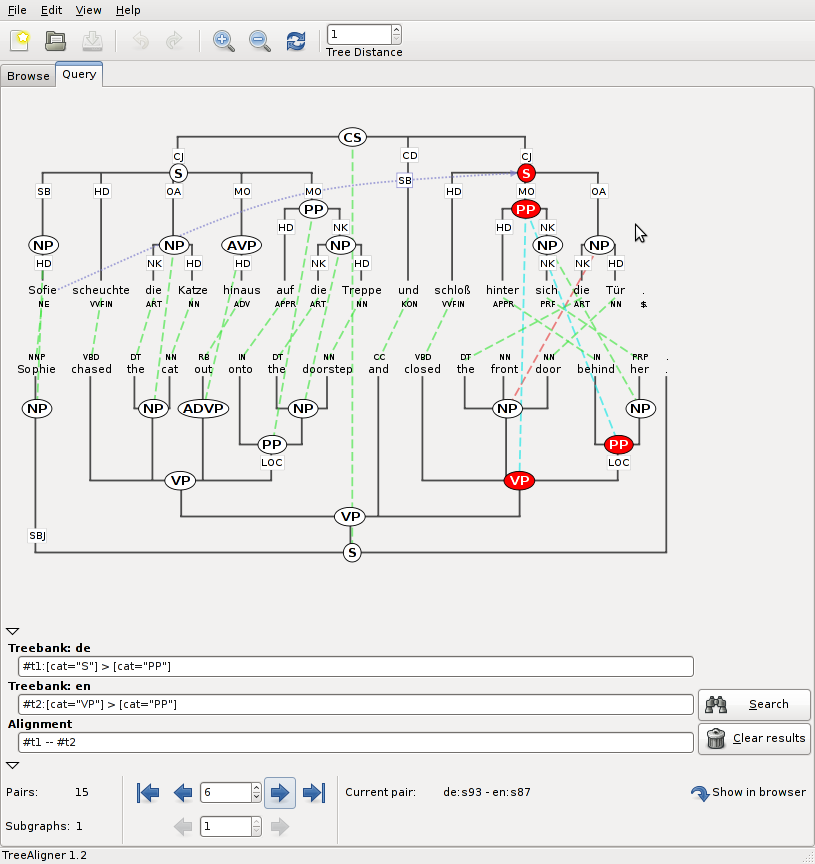
\includegraphics[width=\textwidth]{figures/VolkMarekSamuelssonF2.png}
\caption{Screenshot of the TreeAligner with the Search Module}
\label{fig:volkmareksamuelsson:2}
\end{figure}

The Search Module in the TreeAligner is intended for any parallel treebank where the monolingual treebanks can be converted into TIGER-XML and where the alignment information can be converted to the S\textsc{multron} XML alignment format. The separation of these parts makes it possible to query each treebank separately as well. The system is divided into a monolingual query facility and an alignment query facility that makes use of the former to perform its job. This design choice made it necessary to (re)implement TIGERSearch, the alignment query facility, and the integration into the TreeAligner. 

We chose to reimplement TIGERSearch in Python which influenced the feature set. Even though the implementation of TIGERSearch is well documented (in \citealt{Lezius2002a} among others) and the Java source codes are available under an Open Source license, the reimplementation is not a trivial task. 

The query language for the alignment constraints is kept simple as well. The user can specify that two linguistic objects must be aligned (with exact alignment or approximate alignment). And such constraints can be combined with \textit{AND} statements into more complex constraints. We cannot foresee all options on how a parallel treebank will be queried. We have therefore focused on a clear design of the Search Module rather than overloading it with features. This will facilitate the integration of more features as they are requested by users. 

\subsubsection{Limitations of the TIGER query language}\label{sec:volk:3.2.1}

While certain limitations of query languages are due to the original design and could only be approximated, other valid queries may simply be missing from the query language. \citet{Lai2004} give a list of seven sample queries that each query formalism should support, regardless of the annotation formalism. 

Here we deal with queries that contain universal quantification, i.e.~selecting a tree by stating constraints over sets of nodes rather than individual nodes. The sample queries contain two examples where this is needed \citep{Lai2004}: 

\begin{itemize}
 \item[Q2.] Find sentences that do not include the word \textit{saw}.  
 \item[Q5.] Find the first common ancestor of sequences of a noun phrase followed by a verb phrase.
\end{itemize}

With the TIGER query language and its implementation TIGERSearch \citep{Lezius2002a}, these queries can only be approximated. The result set generated for the approximated queries will likely contain errors. 

Because of the technical nature of the discussion in this section we speak of syntax \textit{graphs} rather than trees. These graphs are directed, acyclic and do not contain structure sharing (i.e.~each node has exactly one direct ancestor). However, due to crossing branches, TIGER trees cannot be stored as nested lists or XML DOM trees directly, which is the usual understanding of trees. 

\textit{Node descriptions} are boolean expressions of feature constraints of the form ``(feature=value)''. They are the basis for finding nodes (assignments) in the corpus which are then used for the constraint resolution in TIGER queries. 

In the TIGER query language, every node variable is implicitly existentially quantified, i.e.~the query 

\ea
\begin{lstlisting}
#s:[cat="S"] !>* #w:[word="saw"] 
\end{lstlisting}
\z

\noindent returns all combinations of two nodes \#s, \#w in all graphs, such that \#s does not dominate \#w (the exclamation mark is the negation operator). From the graphs that were requested in Q2, it will only contain the graphs that do contain the word \textit{saw} outside of an S node. All graphs that do not contain any \textit{saw} will not show up in the result set. Another attempt to formulate Q2 is the query 

\ea
\begin{lstlisting}
#s:[cat="S"] >* #w:[word!="saw"] 
\end{lstlisting}
\z
 
\noindent which returns all combinations of all words except \textit{saw} that are dominated by an S node. 
 
\citet{Lezius2002b} already acknowledges this restriction and proposes to extend the TIGER query formalism with a universal quantifier and the implication operator. While this is natural given the unification-based evaluation of queries in TIGERSearch, an implementation comes at great computational cost. For each universal quantifier in a query, all nodes in the graph have to be iterated to find out if they satisfy the implication. 

\subsubsection{Extensions of the query language in the TreeAligner}\label{sec:volk:3.2.2}

The solution suggested by \citet{Lezius2002b} builds upon the query calculus that is at the core of TIGERSearch's query evaluation engine. In contrast, the query engine in the TreeAligner is based on node sets, and combinations of nodes from the different sets to satisfy the constraints given in a query. We summarize our approach in the following. More details can be found in \citet{MarekEtAl2008}. 

In the previous analysis of Q2, we showed that it is possible to rephrase the query using logical equivalents. Therefore, the query ``get all S nodes that do not contain the word \textit{saw} '' can be rephrased into ``get all graphs where all instances of \textit{saw}, if any, are not dominated by a specific S node''. We already demonstrated that it is not possible to express this query within the old formalism, because one of the operands (``all instances of \textit{saw}, if any'') is a \textit{set} of nodes rather than a single node. In order to get correct results, we introduce a new type into the query language: the node set. 

\subsubsection{Node Sets}\label{sec:volk:3.2.3}

Traditional node descriptions are still bound by an existential quantifier. A node set, in contrast, is bound by a variable that starts with a percentage symbol:

\ea
\begin{lstlisting}
#s:[cat="S"] !>* %w:[word="saw"] 
\end{lstlisting}
\z

If one operand in a constraint is a node set instead of a node, the semantics of the constraint are changed. In this case, only those assignments to \#s are returned where the constraint holds for each node in the node set \%w. In the example at hand, only those S nodes are returned that do not dominate any word \textit{saw} in a graph. 

The semantics of the node predicates that are defined in the TIGER query language do not change, they still operate at the node level. In the query

\ea
\begin{lstlisting}
%np:[cat="NP"] & tokenarity(%np, 2)
\end{lstlisting}
\z

\noindent the node set \%np will contain all NPs whose token arity is 2. In other words, the query matches all NPs that consist of two tokens (e.g.~``\textit{Cash flow}'' or ``\textit{this increase}''). 

If each variable is bound by an existential quantifier, evaluation of a query (or rather, one term in a query in Disjunctive Normal Form) can terminate as soon as one node description does not yield any results. Graphs that do not contain matching nodes for any of the descriptions will also be disregarded. In the presence of node sets, this behavior is wrong. But graphs without any occurrence of \textit{saw} are valid results for the query. Because of that, the semantics of node descriptions bound to node sets are changed. In contrast to nodes, which may not be undefined, they can be the empty set. If this is the case, a constraint is trivially true. 

With this change in place, TIGER is in Cantor's paradise, and no one shall expel it from there. With the basic semantics of set types defined, new set predicates can be introduced to refine queries. As an example, consider the query ``Return all NPs that do not contain any prepositional phrase PP, but only if the graph contains PPs''. With empty node sets allowed, the query would have to be written as

\ea
\begin{lstlisting}
[cat="NP"] !>* %pp:[cat="PP"] & [cat="PP"] 
\end{lstlisting}
\z

\noindent to ensure that at least one PP exists. As a side effect, the result set contains one entry for each combination of NP and PP in a matching graph, which is slightly more than what the query was supposed to yield. If a node set must not be empty, set algebra operations like cardinality, element containment, union and intersection could be added to TIGER. 

Instead of adding support for set operations, we introduced two new predicates that operate exclusively on node sets: \textit{empty} and \textit{nonempty}. The semantics of the predicates can be inferred from the names, and the previous query can be written in a straightforward manner:

\ea
\begin{lstlisting}
[cat="NP"] !>* %pp:[cat="PP"] & nonempty(%pp)
\end{lstlisting}
\z

This makes it possible to search for graphs that do not contain a specific kind of nodes by using the predicate \textit{empty}. The query

\ea
\begin{lstlisting}
%w:[pos="DT"] & empty(%w)
\end{lstlisting}
\z

\noindent returns all graphs that do not contain any determiner. For example, in our S\textsc{multron} economy treebank we find determinerless English headlines such as ``\textit{Group orders grew 8 percent, revenues 10 percent}''. 

\section{Conclusions}\label{sec:volk:4}

We have shown that building parallel treebanks is a complex process. For our \textsc{Smultron} treebank we have used separate tools for creating the monolingual treebanks and the alignment. We have improved the process by automatic treebank deepening, interactive visualisation tools, automatic alignment suggestions and consistency checking over trees and alignments. 

Still, the process remains burdensome in particular since the alignments constitute semantic annotations. We have shown that good alignment guidelines are important. Our experiments have helped us to realize that the guidelines need to contain a host of fine-grained alignment rules and illustrative examples to clarify critical cases. 

Our alignment work would have been impossible without the TreeAligner, our tool for interactive alignment and searching of parallel treebanks. The alignment module provides for quick drag-and-click alignments and supports various views on the aligned trees. The search module allows powerful treebank searches combining constraints over trees and alignments. We have implemented a query language that was inspired by TIGERSearch but which supersedes TIGERSearch with support for universal quantification. 

Future research may go in various directions. We would like to move from a split development of monolingual treebanks and subsequent alignment to a more integrated development process. This should include annotation projection and cross-language consistency checks in every phase of the development process. Moreover recent work on automatic word and phrase alignment should be better integrated into the TreeAligner. 

Annotating a parallel treebank is labor-intensive, but it provides such a wealth of cross-language observations that make it worthwhile and rewarding. 

\section*{Acknowledgments}\label{sec:volk:5}

We gratefully acknowledge financial support for the Smultron project by Granholms stiftelse, Rausings stiftelse and the University of Zurich.

{\sloppy 
\printbibliography[heading=subbibliography,notkeyword=this]
}
\end{document}















